\documentclass[9pt,a4paper,unknownkeysallowed,xcolor=dvipsnames,aspectratio=43]{beamer}
\usepackage{lastpage}
\usepackage{graphicx}
\usepackage{hyperref}  
\usepackage{bm,amsmath,amssymb}

%\usepackage[dvipsnames]{xcolor}
\definecolor{darkred}{RGB}{212, 0, 0}
\definecolor{darkgreen}{RGB}{0,128,0}
\definecolor{teablue}{RGB}{67,0,181}
\definecolor{darkblue}{RGB}{0,0,128}
\hypersetup{
    colorlinks=true,
    linkcolor=blue,
    filecolor=magenta,      
    urlcolor=blue,
    citecolor=blue
}
\newcommand{\currentpage}{\thepage / \pageref{LastPage}}
\setbeamertemplate{footline}
{
  \leavevmode%
  \hbox{%
\footnotesize\sffamily
  \begin{beamercolorbox}[wd=.40\paperwidth,ht=3ex,dp=1ex,center]{}%
   \color{teablue} Jet Physics
  \end{beamercolorbox}%
  \begin{beamercolorbox}[wd=.20\paperwidth,ht=3ex,dp=1ex,center]{}%
  \currentpage 
  \end{beamercolorbox}%
  \begin{beamercolorbox}[wd=.40\paperwidth,ht=3ex,dp=1ex,center]{}%
   \color{teablue} 3. Jet Algorithms
  \end{beamercolorbox}%
}
}
\setbeamertemplate{frametitle}[default][center]
\begin{document}


\begin{frame}
\topskip0pt
\vspace*{\fill}
\begin{center}
{\Huge\bf\color{darkred} Introduction to Jet Physics}\\
\vspace{4mm}
    Bin Wu\\
    \vspace{8mm}
    {\bf\Large Lecture 3: Jet Algorithms}\\\vspace{4mm}
    {\color{darkblue} 16-04-2021}
\end{center}
\vspace{4mm}
\begin{itemize}
    \item[\color{darkred}\Large\bullet] Jet definition
    \vspace{2mm}
    \item[\color{darkred}\Large\bullet] Recombination schemes
    \vspace{2mm}
    \item[\color{darkred}\Large\bullet] Sequential recombination algorithms
    \vspace{2mm}
    \item[\color{darkred}\Large\bullet] Infrared and collinear safety
    \vspace{2mm}
    \item[\color{darkred}\Large\bullet] Jet algorithms as optimization problem

\end{itemize}
\vspace*{\fill}
\end{frame}
%
%%%%%%%%%%%%%%%%%%%%%%%%%%%%%%%%%%%%%%%%%%%%%%%%%%%%%%%%%%
%
\begin{frame}{\bf\huge Jet definition}

{\color{darkred}\Large$\bullet$} A jet definition:
\begin{center}
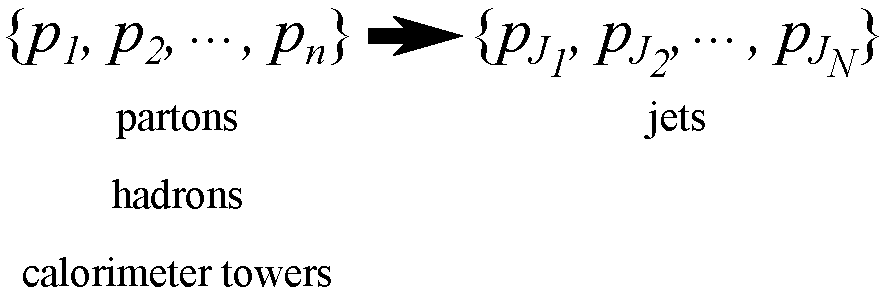
\includegraphics[width=0.5\textwidth]{03/jetdef.pdf}
\end{center}
\begin{itemize}
    \item[\diamondsuit] {\color{darkred} Jet Algorithm:} how to group particles into jets
    \vspace{1mm}
    \item[\diamondsuit] {\color{darkred} Recombination scheme:} how to define $p_{J_i}$ from the constituents of $J_i$
\end{itemize}
\vspace{2mm}

{\color{darkred}\Large$\bullet$} {\color{darkred}The Snowmass accord:} a jet definition meets the following properties
\vspace{2mm}
\begin{enumerate}
  \itemsep-0.1cm
\item Simple to implement in an experimental analysis;\vspace{2mm}
\item Simple to implement in the theoretical calculation;\vspace{2mm}
\item Defined at any order of perturbation theory;\vspace{2mm}
\item Yields finite cross sections at any order of perturbation theory;\vspace{2mm}
\item Yields a cross section that is relatively insensitive to hadronisation.
\end{enumerate}
\end{frame}

%
%%%%%%%%%%%%%%%%%%%%%%%%%%%%%%%%%%%%%%%%%%%%%%%%%%%%%%%%%%
%
\begin{frame}{\bf\huge The recombination schemes}

{\color{darkred}\Large$\bullet$} {\color{darkred}A recombination scheme} tells us how to combine the momenta of the constituents of a jet.\\
\vspace{2mm}

{\color{darkred}\Large$\bullet$} Recombination schemes suggested for hadron colliders include:
\begin{enumerate}
    \item {\color{darkred}The E-scheme} (four-momentum combination scheme): 
    \begin{align}
    p^\mu_i, p^\mu_j \to p^\mu_{r}=p^\mu_i + p^\mu_j.
    \end{align}
    \item {\color{darkred}The winner-take-all (WTA) scheme:} 
    \begin{align}
    &p_{T, r} = p_{T, i} + p_{T, j}\notag\\
    &\text{$(y_r, \phi_r, m_r)$ = $(y, \phi, m)$ of the particle with larger $p_T$}
    \end{align}
    \item {\color{darkred}Other schemes:}
    \begin{align}
    &p_{T, r} = p_{T, i} + p_{T, j},\qquad \phi_r = \frac{\omega_i \phi_i + \omega_j \phi_j}{\omega_i + \omega_j},\qquad y_r = \frac{\omega_i y_i + \omega_j y_j}{\omega_i + \omega_j} 
    \end{align}
    with
    \begin{ali}
    \omega_i = \left\{\begin{array}{ll}
         p_{T, i}&  \text{for the $p_T$ and $E_T$ scheme}\\
         p^2_{T, i}&  \text{for the $p_T^2$ and $E_T^2$ scheme}
    \end{array}
    \right..
    \end{ali}
\end{enumerate}
\end{frame}
%
%%%%%%%%%%%%%%%%%%%%%%%%%%%%%%%%%%%%%%%%%%%%%%%%%%%%%%%%%%
%
\begin{frame}{\bf\huge Sequential recombination algorithms}

{\color{darkred}\Large$\bullet$} Aim: to invert the successive parton branchings that produce jets.\\
\vspace{2mm}

{\color{darkred}\Large$\bullet$} Recall that the branching is enhanced in collinear and soft limit:
\begin{align}
    P_r=\frac{\alpha_s C_F}{\pi^2}\int\frac{d\omega}{\omega}\frac{d^2k_\perp}{k_\perp^2} = \frac{\alpha_s C_F}{\pi^2}\int\frac{d\omega}{\omega}\frac{d\Delta \Omega}{\Delta \Omega}=\frac{2\alpha_s C_F}{\pi^2}\int\frac{d\omega}{\omega}\frac{d\sqrt{\Delta \Omega}}{\sqrt{\Delta \Omega}}
\end{align}
\begin{center}
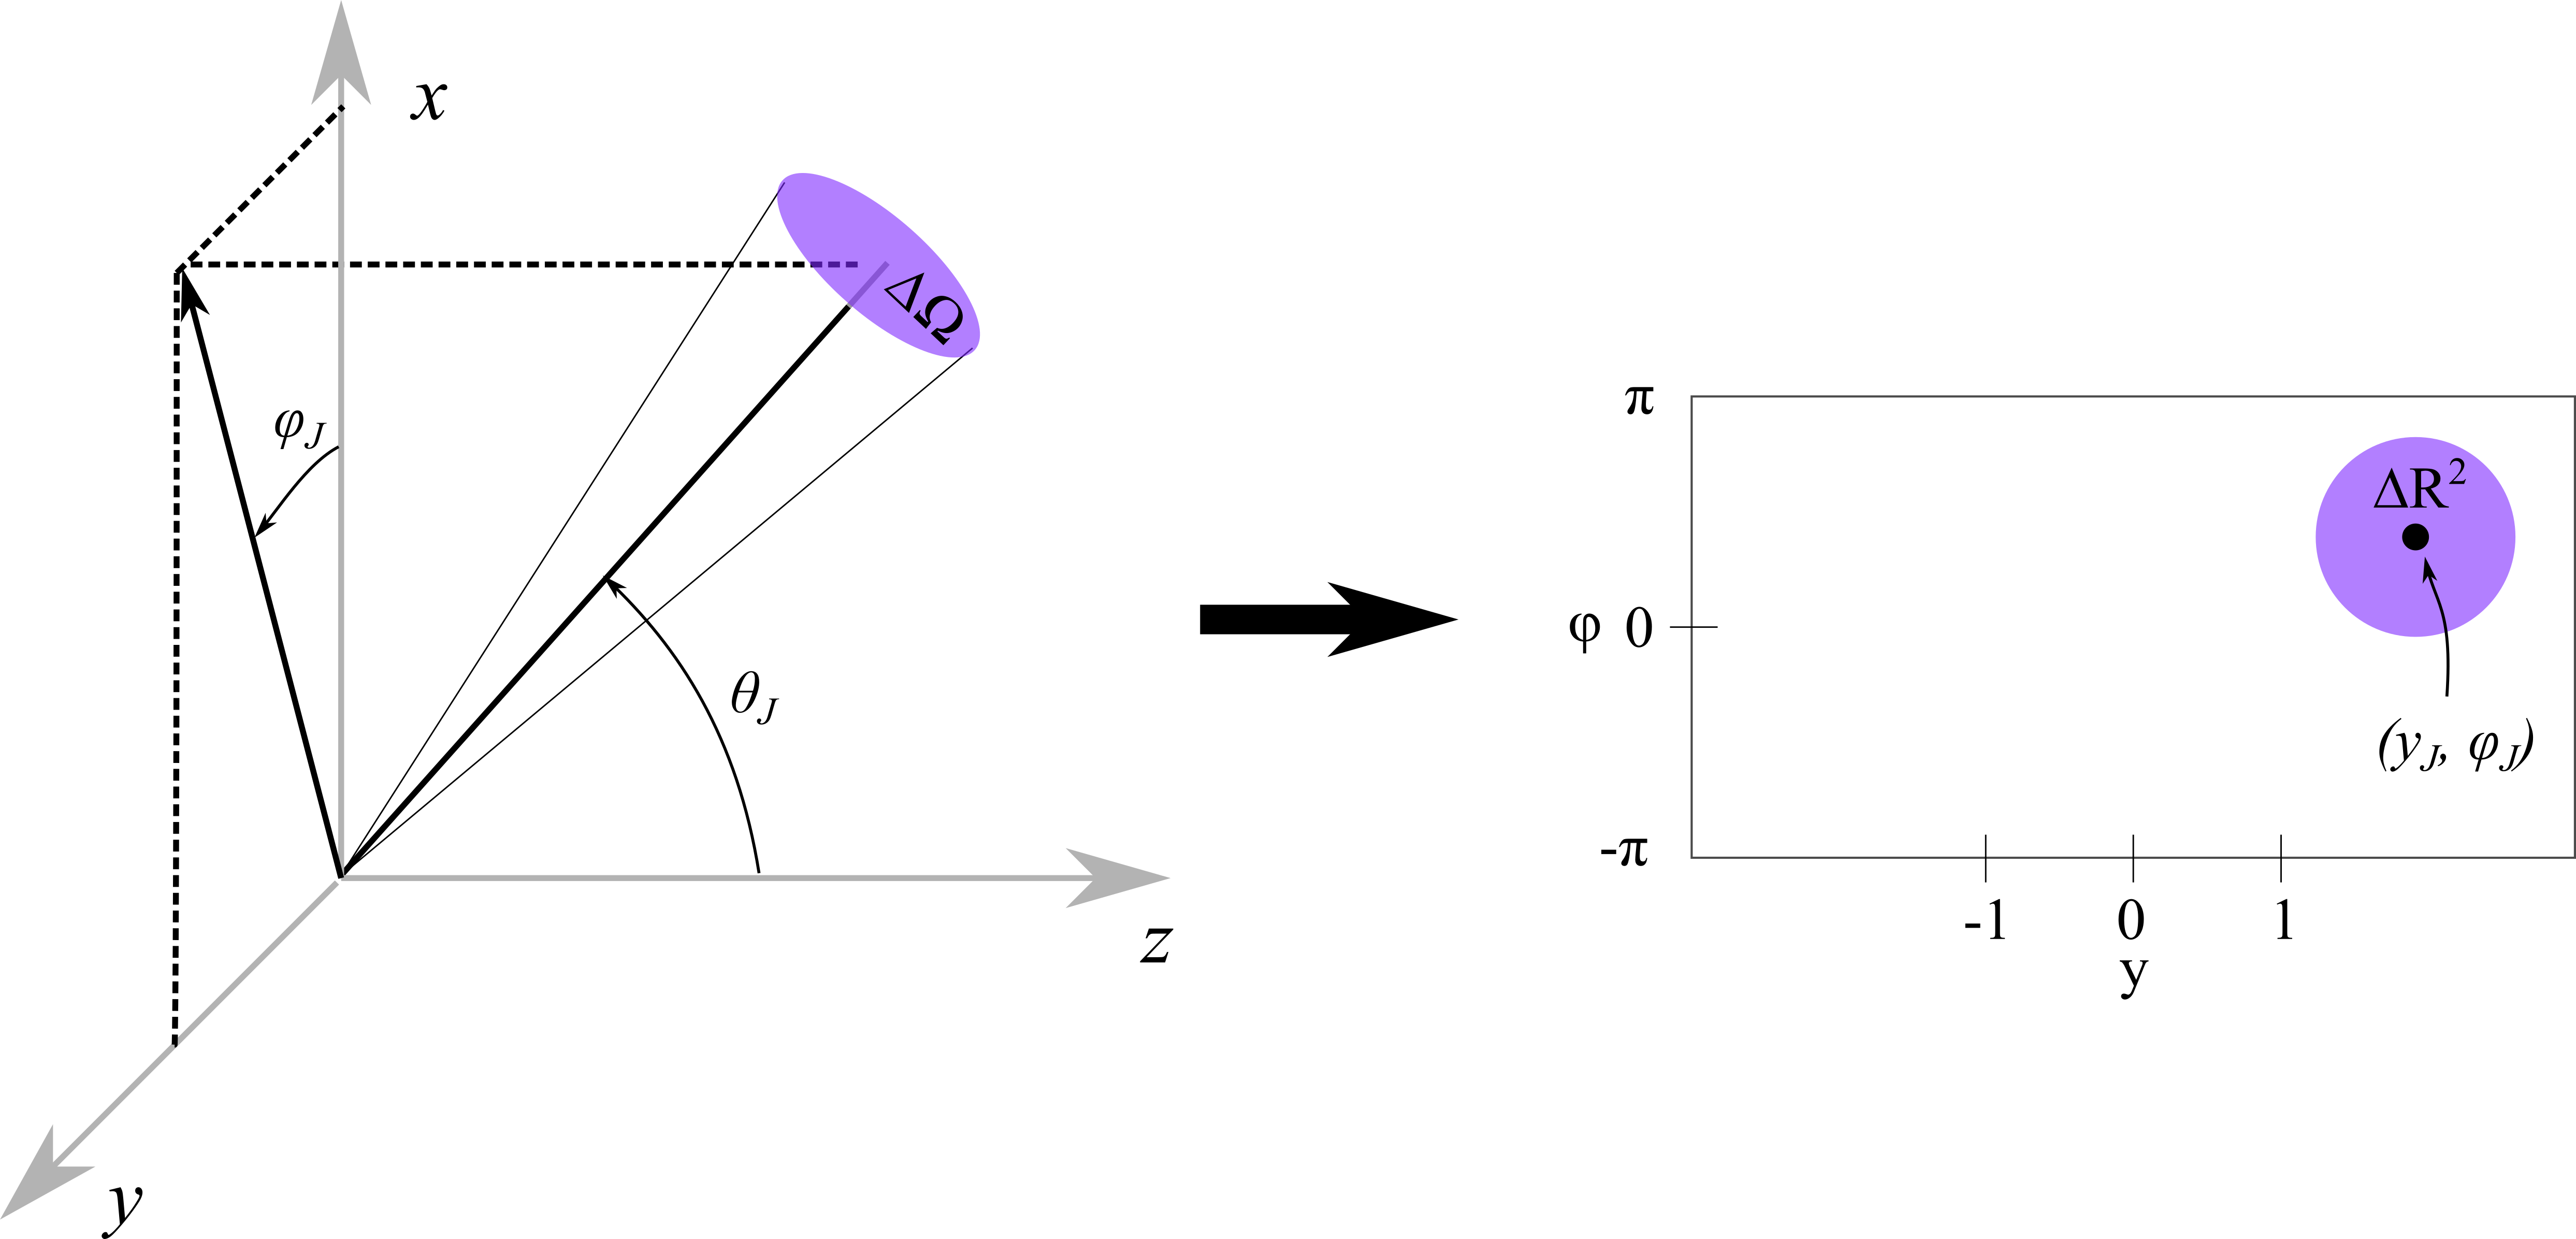
\includegraphics[width=0.65\textwidth]{R.png}
\end{center}
\begin{align}
\Delta \Omega = \Delta R^2/\cosh y    
\end{align}
Therefore, the smaller $k_T \Delta R$ is, the more likely a parton radiates.
\end{frame}
%
%%%%%%%%%%%%%%%%%%%%%%%%%%%%%%%%%%%%%%%%%%%%%%%%%%%%%%%%%%
%
\begin{frame}

{\color{darkred}\Large$\bullet$} This motives the use of {\color{darkred} $k_t$ algorithm}, in which one defines 
an {\em inter-particle distance}
  \begin{equation}
    d_{ij} = \text{min}(p_{T,i}^{2},p_{T,j}^{2}) \frac{\Delta R_{ij}^2}{R^2},
  \end{equation}
and
a {\em beam distance}
  \begin{equation}
    d_{iB} = p_{T,i}^{2},
  \end{equation}
  with $R$ a free parameter called the {\em jet radius}.
 \vspace{2mm}
  
{\color{darkred}\Large$\bullet$} The list of jets is clustered from the list of particles, named {\it pseudojet}:
\vspace{2mm}
\begin{enumerate}
\item Identify the smallest of the $d_{ij}$ and $d_{iB}$.
  \vspace{2mm}
  \begin{itemize}
  \item[\diamondsuit] If the smallest distance is a $d_{ij}$, replace $i$ and
    $j$ with a new pseudojet of momentum $p_r$ given as a function of $p_i, p_j$ according to some recombination scheme.
    \vspace{2mm}
    
  \item[\diamondsuit] If the smallest is a $d_{iB}$, declare $i$ is a {\em jet} and remove it from the list.
  \end{itemize}
  \item If the list of pseudojets is not empty, go back to step 1 until all the objects in the list have
  been exhausted.
\end{enumerate}
\vspace{2mm}

{\color{darkred}\Large$\bullet$} Two parameters: $R$ and $p_{T,min}$. One only uses jets with $p_T > p_{T,min}$.

\end{frame}
%
%%%%%%%%%%%%%%%%%%%%%%%%%%%%%%%%%%%%%%%%%%%%%%%%%%%%%%%%%%
%
\begin{frame}\vspace{2mm}

{\color{darkred}\Large$\bullet$} An example: group 5 massless particles to jets with $R=1$:
\begin{align}
(p_T, y, \phi) = &{\color{red}(100, 0.8, 0)}, {\color{blue}(100, -0.8, 0)},\notag\\
&{\color{magenta}(1, 0.3, 0), (10, -0.15, -0.1), (8, 0.3, 0.6)}.\notag
\end{align}

{\color{darkred}\Large$\bullet$} How are {\color{magenta}soft particles} recombined with two hard ones ({\color{red}red} and {\color{blue}blue})?
\vspace{2mm}
\begin{center}
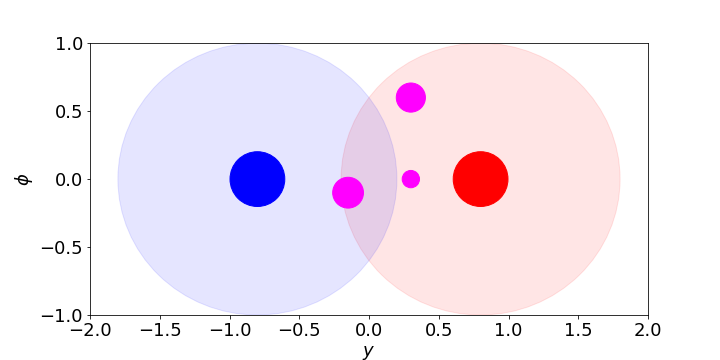
\includegraphics[width=0.8\textwidth]{kt0.png}
\end{center}
\end{frame}
%
%%%%%%%%%%%%%%%%%%%%%%%%%%%%%%%%%%%%%%%%%%%%%%%%%%%%%%%%%%
%
\begin{frame}\vspace{2mm}

{\color{darkred}\Large$\bullet$} An example: group 5 massless particles to jets with $R=1$:
\begin{align}
(p_T, y, \phi) = &{\color{red}(100, 0.8, 0)}, {\color{blue}(100, -0.8, 0)},\notag\\
&{\color{magenta}(1, 0.3, 0), (10, -0.15, -0.1), (8, 0.3, 0.6)}.\notag
\end{align}

{\color{darkred}\Large$\bullet$} Step 1:
\vspace{2mm}
\begin{center}
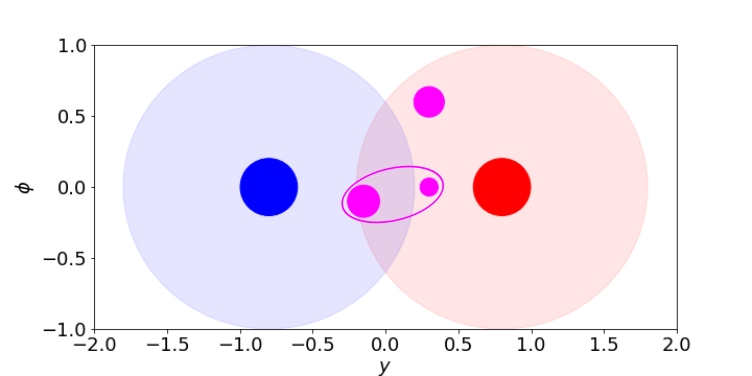
\includegraphics[width=0.8\textwidth]{kt01.png}
\end{center}
\end{frame}

%
%%%%%%%%%%%%%%%%%%%%%%%%%%%%%%%%%%%%%%%%%%%%%%%%%%%%%%%%%%
%
\begin{frame}\vspace{2mm}

{\color{darkred}\Large$\bullet$} An example: group 5 massless particles to jets with $R=1$:
\begin{align}
(p_T, y, \phi) = &{\color{red}(100, 0.8, 0)}, {\color{blue}(100, -0.8, 0)},\notag\\
&{\color{magenta}(1, 0.3, 0), (10, -0.15, -0.1), (8, 0.3, 0.6)}.\notag
\end{align}

{\color{darkred}\Large$\bullet$} Step 1:
\vspace{2mm}
\begin{center}
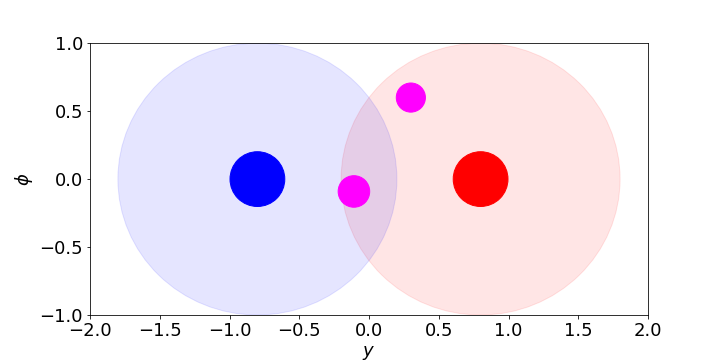
\includegraphics[width=0.8\textwidth]{kt1.png}
\end{center}
\end{frame}
%
%%%%%%%%%%%%%%%%%%%%%%%%%%%%%%%%%%%%%%%%%%%%%%%%%%%%%%%%%%
%
\begin{frame}\vspace{2mm}

{\color{darkred}\Large$\bullet$} An example: group 5 massless particles to jets with $R=1$:
\begin{align}
(p_T, y, \phi) = &{\color{red}(100, 0.8, 0)}, {\color{blue}(100, -0.8, 0)},\notag\\
&{\color{magenta}(1, 0.3, 0), (10, -0.15, -0.1), (8, 0.3, 0.6)}.\notag
\end{align}

{\color{darkred}\Large$\bullet$} Step 2:
\vspace{2mm}
\begin{center}
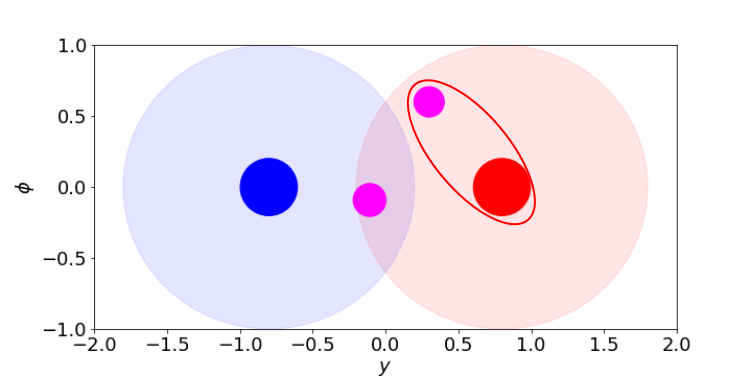
\includegraphics[width=0.8\textwidth]{kt12.png}
\end{center}
\end{frame}
%
%
%%%%%%%%%%%%%%%%%%%%%%%%%%%%%%%%%%%%%%%%%%%%%%%%%%%%%%%%%%
%
\begin{frame}\vspace{2mm}

{\color{darkred}\Large$\bullet$} An example: group 5 massless particles to jets with $R=1$:
\begin{align}
(p_T, y, \phi) = &{\color{red}(100, 0.8, 0)}, {\color{blue}(100, -0.8, 0)},\notag\\
&{\color{magenta}(1, 0.3, 0), (10, -0.15, -0.1), (8, 0.3, 0.6)}.\notag
\end{align}

{\color{darkred}\Large$\bullet$} Step 2:
\vspace{2mm}
\begin{center}
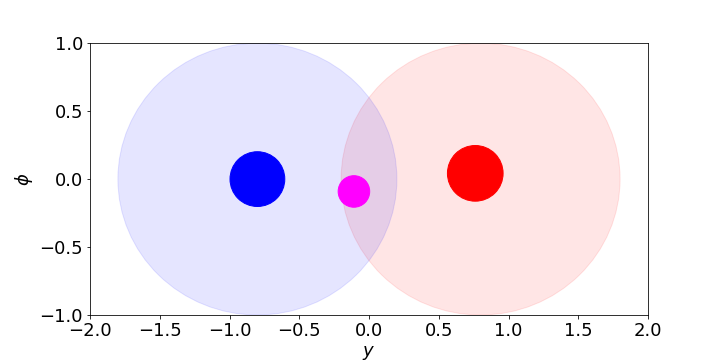
\includegraphics[width=0.8\textwidth]{kt2.png}
\end{center}
\end{frame}
%
%%%%%%%%%%%%%%%%%%%%%%%%%%%%%%%%%%%%%%%%%%%%%%%%%%%%%%%%%%
%
\begin{frame}\vspace{2mm}

{\color{darkred}\Large$\bullet$} An example: group 5 massless particles to jets with $R=1$:
\begin{align}
(p_T, y, \phi) = &{\color{red}(100, 0.8, 0)}, {\color{blue}(100, -0.8, 0)},\notag\\
&{\color{magenta}(1, 0.3, 0), (10, -0.15, -0.1), (8, 0.3, 0.6)}.\notag
\end{align}

{\color{darkred}\Large$\bullet$} Step 3:
\vspace{2mm}
\begin{center}
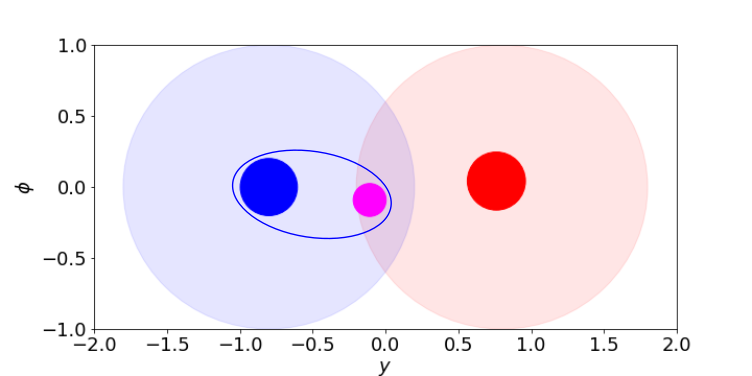
\includegraphics[width=0.8\textwidth]{kt23.png}
\end{center}
\end{frame}
%
%%%%%%%%%%%%%%%%%%%%%%%%%%%%%%%%%%%%%%%%%%%%%%%%%%%%%%%%%%
%
\begin{frame}\vspace{2mm}

{\color{darkred}\Large$\bullet$} An example: group 5 massless particles to jets with $R=1$:
\begin{align}
(p_T, y, \phi) = &{\color{red}(100, 0.8, 0)}, {\color{blue}(100, -0.8, 0)},\notag\\
&{\color{magenta}(1, 0.3, 0), (10, -0.15, -0.1), (8, 0.3, 0.6)}.\notag
\end{align}

{\color{darkred}\Large$\bullet$} Step 3: one ends up with a dijet event
\vspace{2mm}
\begin{center}
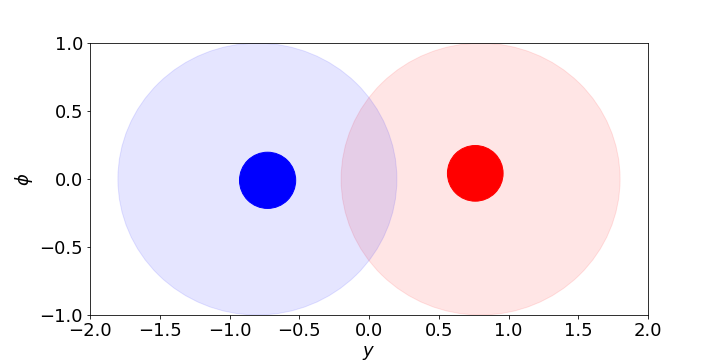
\includegraphics[width=0.8\textwidth]{kt3.png}
\end{center}
\end{frame}
%
%%%%%%%%%%%%%%%%%%%%%%%%%%%%%%%%%%%%%%%%%%%%%%%%%%%%%%%%%%
%
\begin{frame}\vspace{2mm}

{\color{darkred}\Large$\bullet$} In summary:
\vspace{2mm}

\begin{center}
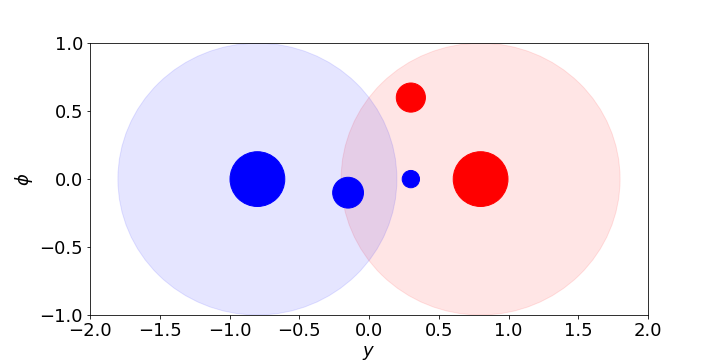
\includegraphics[width=0.8\textwidth]{03/ktcls.png}
\end{center}
\vspace{2mm}

{\color{darkred}\Large$\bullet$} $k_t$ algorithm has the {\color{darkred}disadvantage} that jets become more sensitive to soft radiation (UE or pileup). And it produces geometrically irregular jets.
\end{frame}
%
%%%%%%%%%%%%%%%%%%%%%%%%%%%%%%%%%%%%%%%%%%%%%%%%%%%%%%%%%%
%
\begin{frame}

{\color{darkred}\Large$\bullet$} In {\color{darkred}generalised-$k_t$ algorithm}, one defines 
an {\em inter-particle distance}
  \begin{equation}
    d_{ij} = \text{min}(p_{T,i}^{2p},p_{T,j}^{2p}) \frac{\Delta R_{ij}^2}{R^2},
  \end{equation}
and
a {\em beam distance}
  \begin{equation}
    d_{iB} = p_{T,i}^{2p}.
  \end{equation}
 \vspace{2mm}
  
  
{\color{darkred}\Large$\bullet$} The list of jets is clustered from the list of particles (pseudojet) in the same way as $k_T$-algorithm, that is,
\vspace{2mm}
\begin{enumerate}
\item Identify the smallest of the $d_{ij}$ and $d_{iB}$.
  \vspace{2mm}
  \begin{itemize}
  \item[\diamondsuit] If the smallest distance is a $d_{ij}$, replace $i$ and
    $j$ with a new pseudojet of momentum $p_r$ given as a function of $p_i, p_j$ according to some recombination scheme.
    \vspace{2mm}
    
  \item[\diamondsuit] If the smallest is a $d_{iB}$, declare $i$ is a {\em jet} and remove it from the list.
  \end{itemize}
  \item If the list of pseudojets is not empty, go back to step 1 until all the objects in the list have
  been exhausted.
\end{enumerate}
\end{frame}
%
%%%%%%%%%%%%%%%%%%%%%%%%%%%%%%%%%%%%%%%%%%%%%%%%%%%%%%%%%%
%
\begin{frame}

{\color{darkred}\Large$\bullet$} {\color{darkred} The Cambridge/Aachen algorithm:}

  \begin{equation}
    d_{ij} = \frac{\Delta R_{ij}^2}{R^2}\qquad d_{iB} = 1.\notag
  \end{equation}
 \vspace{2mm}
  
{\color{darkred}\Large$\bullet$} Go back to the same 5 particles:
\vspace{2mm}
\begin{center}
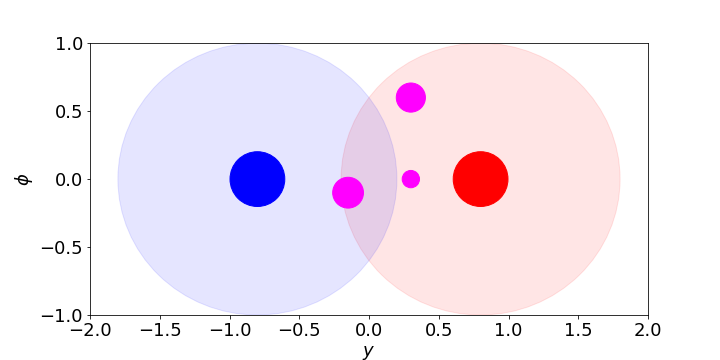
\includegraphics[width=0.8\textwidth]{kt0.png}
\end{center}
\end{frame}
%
%%%%%%%%%%%%%%%%%%%%%%%%%%%%%%%%%%%%%%%%%%%%%%%%%%%%%%%%%%
%
\begin{frame}

{\color{darkred}\Large$\bullet$} {\color{darkred} The Cambridge/Aachen algorithm:}

  \begin{equation}
    d_{ij} = \frac{\Delta R_{ij}^2}{R^2}\qquad d_{iB} = 1.\notag
  \end{equation}
 \vspace{2mm}
  
{\color{darkred}\Large$\bullet$} Step 1:
\vspace{2mm}
\begin{center}
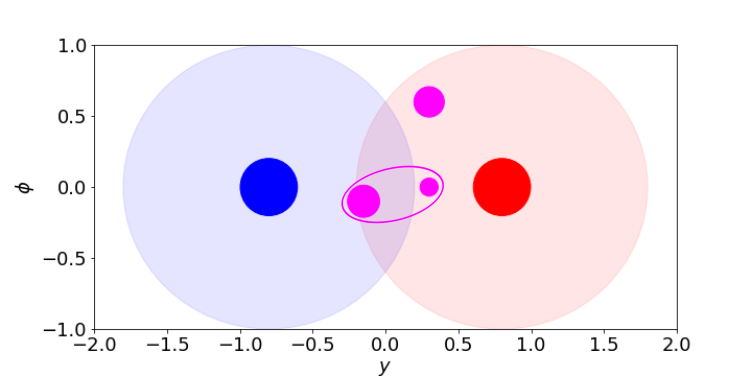
\includegraphics[width=0.8\textwidth]{ca01.png}
\end{center}
\end{frame}
%
%%%%%%%%%%%%%%%%%%%%%%%%%%%%%%%%%%%%%%%%%%%%%%%%%%%%%%%%%%
%
\begin{frame}

{\color{darkred}\Large$\bullet$} {\color{darkred} The Cambridge/Aachen algorithm:}

  \begin{equation}
    d_{ij} = \frac{\Delta R_{ij}^2}{R^2}\qquad d_{iB} = 1.\notag
  \end{equation}
 \vspace{2mm}
  
{\color{darkred}\Large$\bullet$} Step 1:
\vspace{2mm}
\begin{center}
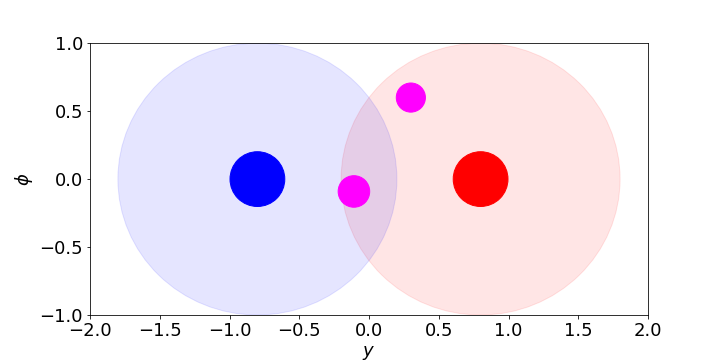
\includegraphics[width=0.8\textwidth]{ca1.png}
\end{center}
\end{frame}
%
%%%%%%%%%%%%%%%%%%%%%%%%%%%%%%%%%%%%%%%%%%%%%%%%%%%%%%%%%%
%
\begin{frame}

{\color{darkred}\Large$\bullet$} {\color{darkred} The Cambridge/Aachen algorithm:}

  \begin{equation}
    d_{ij} = \frac{\Delta R_{ij}^2}{R^2}\qquad d_{iB} = 1.\notag
  \end{equation}
 \vspace{2mm}
  
{\color{darkred}\Large$\bullet$} Step 2:
\vspace{2mm}
\begin{center}
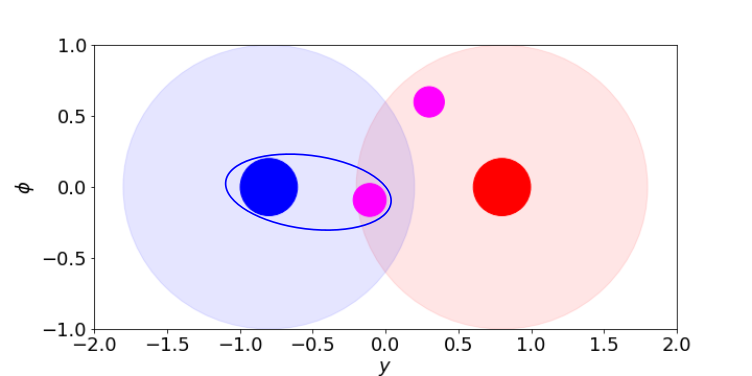
\includegraphics[width=0.8\textwidth]{ca12.png}
\end{center}
\end{frame}
%
%%%%%%%%%%%%%%%%%%%%%%%%%%%%%%%%%%%%%%%%%%%%%%%%%%%%%%%%%%
%
\begin{frame}

{\color{darkred}\Large$\bullet$} {\color{darkred} The Cambridge/Aachen algorithm:}

  \begin{equation}
    d_{ij} = \frac{\Delta R_{ij}^2}{R^2}\qquad d_{iB} = 1.\notag
  \end{equation}
 \vspace{2mm}
  
{\color{darkred}\Large$\bullet$} Step 2:
\vspace{2mm}
\begin{center}
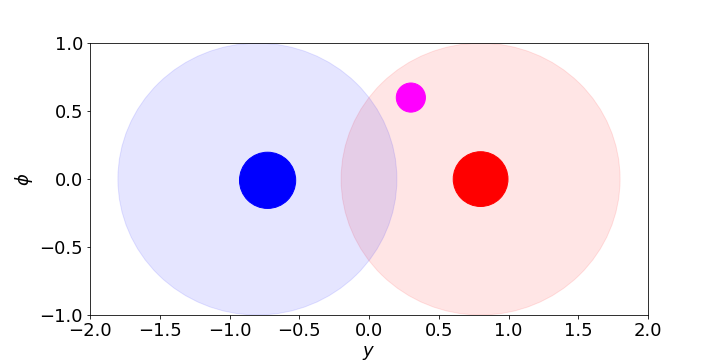
\includegraphics[width=0.8\textwidth]{ca2.png}
\end{center}
\end{frame}
%
%%%%%%%%%%%%%%%%%%%%%%%%%%%%%%%%%%%%%%%%%%%%%%%%%%%%%%%%%%
%
\begin{frame}

{\color{darkred}\Large$\bullet$} {\color{darkred} The Cambridge/Aachen algorithm:}

  \begin{equation}
    d_{ij} = \frac{\Delta R_{ij}^2}{R^2}\qquad d_{iB} = 1.\notag
  \end{equation}
 \vspace{2mm}
  
{\color{darkred}\Large$\bullet$} Step 3:
\vspace{2mm}
\begin{center}
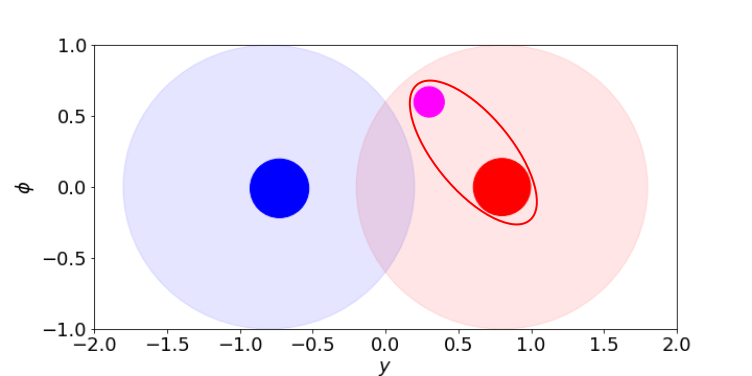
\includegraphics[width=0.8\textwidth]{ca23.png}
\end{center}
\end{frame}
%
%%%%%%%%%%%%%%%%%%%%%%%%%%%%%%%%%%%%%%%%%%%%%%%%%%%%%%%%%%
%
\begin{frame}

{\color{darkred}\Large$\bullet$} {\color{darkred} The Cambridge/Aachen algorithm:}

  \begin{equation}
    d_{ij} = \frac{\Delta R_{ij}^2}{R^2}\qquad d_{iB} = 1.\notag
  \end{equation}
 \vspace{2mm}
  
{\color{darkred}\Large$\bullet$} Step 3:
\vspace{2mm}
\begin{center}
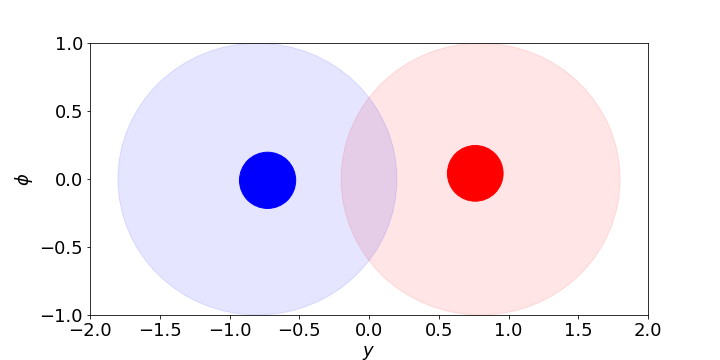
\includegraphics[width=0.8\textwidth]{ca3.png}
\end{center}
\end{frame}
%
%%%%%%%%%%%%%%%%%%%%%%%%%%%%%%%%%%%%%%%%%%%%%%%%%%%%%%%%%%
%
\begin{frame}

{\color{darkred}\Large$\bullet$} {\color{darkred} The Cambridge/Aachen algorithm:}

  \begin{equation}
    d_{ij} = \frac{\Delta R_{ij}^2}{R^2}\qquad d_{iB} = 1.\notag
  \end{equation}
 \vspace{2mm}
  
{\color{darkred}\Large$\bullet$} In summary:
\vspace{2mm}
\begin{center}
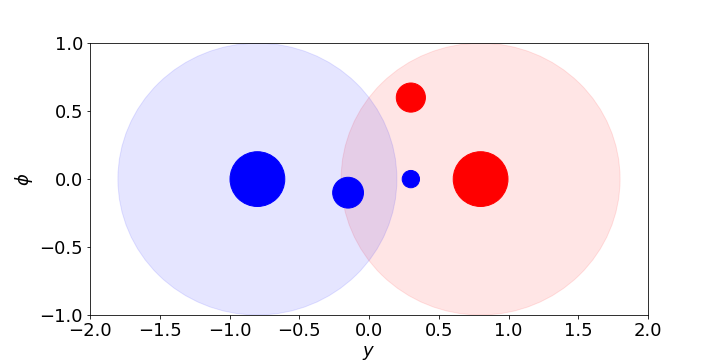
\includegraphics[width=0.8\textwidth]{cacls.png}
\end{center}
\end{frame}
%
%%%%%%%%%%%%%%%%%%%%%%%%%%%%%%%%%%%%%%%%%%%%%%%%%%%%%%%%%%
%
\begin{frame}

{\color{darkred}\Large$\bullet$} {\color{darkred} At the LHC, jets are almost always defined with the anti-$k_t$ algorithm:}

  \begin{equation}
    d_{ij} = \text{min}(p_{T,i}^{-2},p_{T,j}^{-2})\frac{\Delta R_{ij}^2}{R^2}\qquad d_{iB} = p_{T,i}^{-2}.
  \notag\end{equation}
 \vspace{2mm}
  
{\color{darkred}\Large$\bullet$} Go back to the same 5 particles:
\vspace{2mm}
\begin{center}
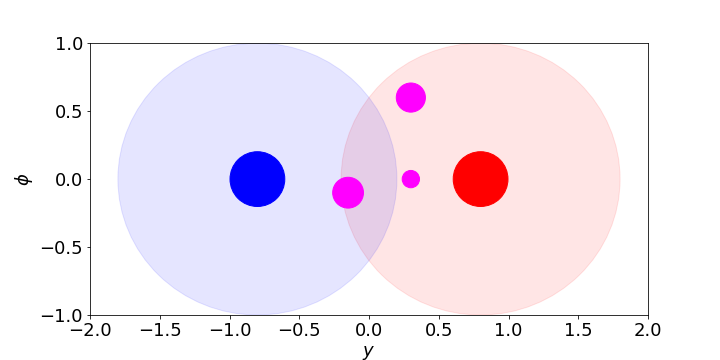
\includegraphics[width=0.8\textwidth]{kt0.png}
\end{center}
\end{frame}
%
%%%%%%%%%%%%%%%%%%%%%%%%%%%%%%%%%%%%%%%%%%%%%%%%%%%%%%%%%%
%
\begin{frame}

{\color{darkred}\Large$\bullet$} {\color{darkred} At the LHC, jets are almost always defined with the anti-$k_t$ algorithm:}

  \begin{equation}
    d_{ij} = \text{min}(p_{T,i}^{-2},p_{T,j}^{-2})\frac{\Delta R_{ij}^2}{R^2}\qquad d_{iB} = p_{T,i}^{-2}.
  \notag\end{equation}
 \vspace{2mm}
  
{\color{darkred}\Large$\bullet$} Step 1:
\vspace{2mm}
\begin{center}
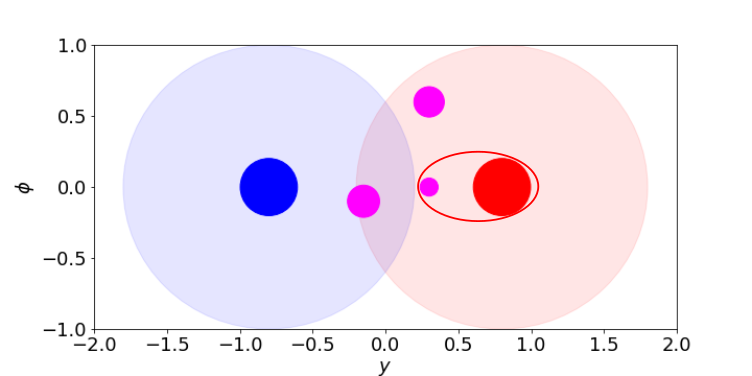
\includegraphics[width=0.8\textwidth]{antikt01.png}
\end{center}
\end{frame}
%
%%%%%%%%%%%%%%%%%%%%%%%%%%%%%%%%%%%%%%%%%%%%%%%%%%%%%%%%%%
%
\begin{frame}

{\color{darkred}\Large$\bullet$} {\color{darkred} At the LHC, jets are almost always defined with the anti-$k_t$ algorithm:}

  \begin{equation}
    d_{ij} = \text{min}(p_{T,i}^{-2},p_{T,j}^{-2})\frac{\Delta R_{ij}^2}{R^2}\qquad d_{iB} = p_{T,i}^{-2}.
  \notag\end{equation}
 \vspace{2mm}
  
{\color{darkred}\Large$\bullet$} Step 1:
\vspace{2mm}
\begin{center}
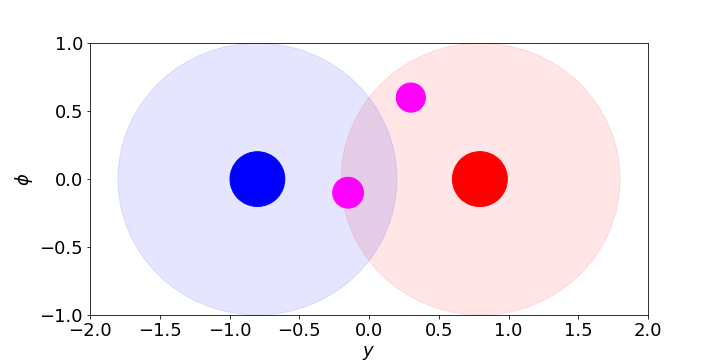
\includegraphics[width=0.8\textwidth]{antikt1.png}
\end{center}
\end{frame}
%
%
%%%%%%%%%%%%%%%%%%%%%%%%%%%%%%%%%%%%%%%%%%%%%%%%%%%%%%%%%%
%
\begin{frame}

{\color{darkred}\Large$\bullet$} {\color{darkred} At the LHC, jets are almost always defined with the anti-$k_t$ algorithm:}

  \begin{equation}
    d_{ij} = \text{min}(p_{T,i}^{-2},p_{T,j}^{-2})\frac{\Delta R_{ij}^2}{R^2}\qquad d_{iB} = p_{T,i}^{-2}.
  \notag\end{equation}
 \vspace{2mm}
  
{\color{darkred}\Large$\bullet$} Step 2:
\vspace{2mm}
\begin{center}
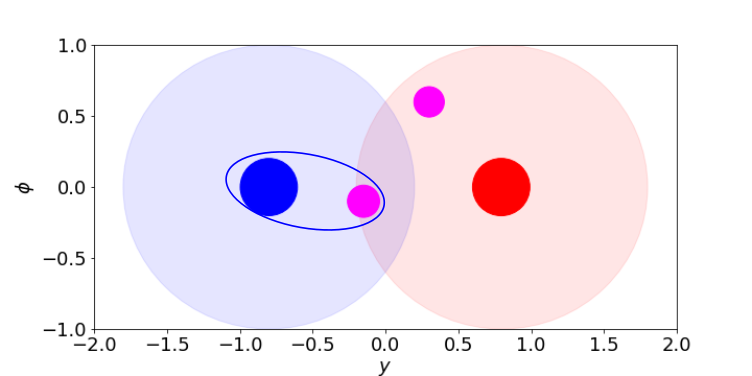
\includegraphics[width=0.8\textwidth]{antikt12.png}
\end{center}
\end{frame}
%
%
%%%%%%%%%%%%%%%%%%%%%%%%%%%%%%%%%%%%%%%%%%%%%%%%%%%%%%%%%%
%
\begin{frame}

{\color{darkred}\Large$\bullet$} {\color{darkred} At the LHC, jets are almost always defined with the anti-$k_t$ algorithm:}

  \begin{equation}
    d_{ij} = \text{min}(p_{T,i}^{-2},p_{T,j}^{-2})\frac{\Delta R_{ij}^2}{R^2}\qquad d_{iB} = p_{T,i}^{-2}.
  \notag\end{equation}
 \vspace{2mm}
  
{\color{darkred}\Large$\bullet$} Step 2:
\vspace{2mm}
\begin{center}
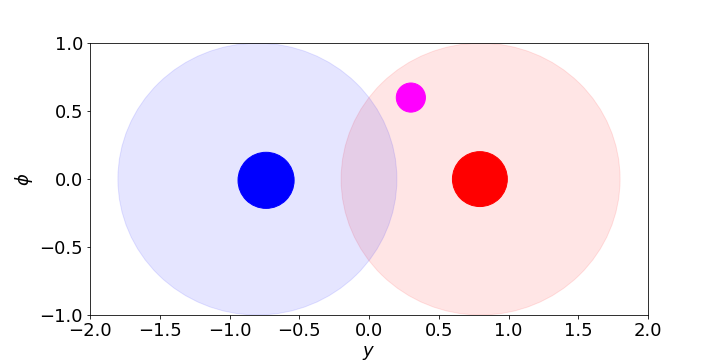
\includegraphics[width=0.8\textwidth]{antikt2.png}
\end{center}
\end{frame}
%
%%%%%%%%%%%%%%%%%%%%%%%%%%%%%%%%%%%%%%%%%%%%%%%%%%%%%%%%%%
%
\begin{frame}

{\color{darkred}\Large$\bullet$} {\color{darkred} At the LHC, jets are almost always defined with the anti-$k_t$ algorithm:}

  \begin{equation}
    d_{ij} = \text{min}(p_{T,i}^{-2},p_{T,j}^{-2})\frac{\Delta R_{ij}^2}{R^2}\qquad d_{iB} = p_{T,i}^{-2}.
  \notag\end{equation}
 \vspace{2mm}
  
{\color{darkred}\Large$\bullet$} Step 3:
\vspace{2mm}
\begin{center}
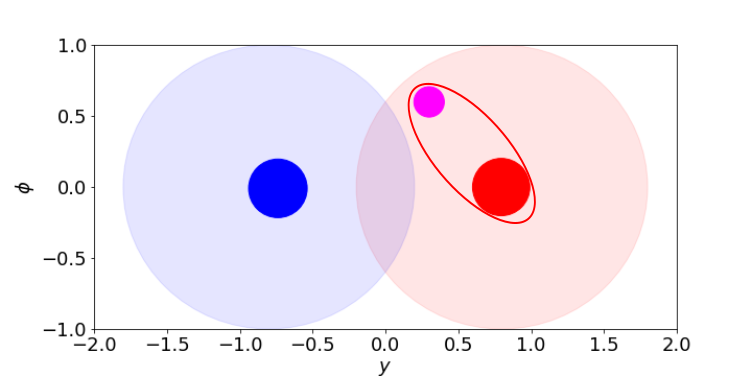
\includegraphics[width=0.8\textwidth]{antikt23.png}
\end{center}
\end{frame}
%
%%%%%%%%%%%%%%%%%%%%%%%%%%%%%%%%%%%%%%%%%%%%%%%%%%%%%%%%%%
%
\begin{frame}

{\color{darkred}\Large$\bullet$} {\color{darkred} At the LHC, jets are almost always defined with the anti-$k_t$ algorithm:}

  \begin{equation}
    d_{ij} = \text{min}(p_{T,i}^{-2},p_{T,j}^{-2})\frac{\Delta R_{ij}^2}{R^2}\qquad d_{iB} = p_{T,i}^{-2}.
  \notag\end{equation}
 \vspace{2mm}
  
{\color{darkred}\Large$\bullet$} Step 3:
\vspace{2mm}
\begin{center}
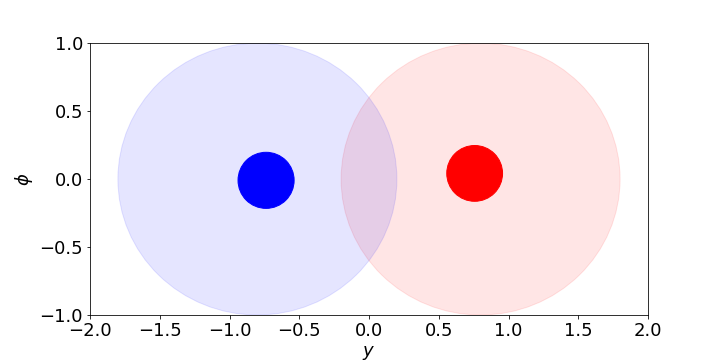
\includegraphics[width=0.8\textwidth]{antikt3.png}
\end{center}
\end{frame}
%
%%%%%%%%%%%%%%%%%%%%%%%%%%%%%%%%%%%%%%%%%%%%%%%%%%%%%%%%%%
%
\begin{frame}

{\color{darkred}\Large$\bullet$} {\color{darkred} At the LHC, jets are almost always defined with the anti-$k_t$ algorithm:}

  \begin{equation}
    d_{ij} = \text{min}(p_{T,i}^{-2},p_{T,j}^{-2})\frac{\Delta R_{ij}^2}{R^2}\qquad d_{iB} = p_{T,i}^{-2}.
  \notag\end{equation}
 \vspace{2mm}
  
{\color{darkred}\Large$\bullet$} In summary:
\vspace{2mm}
\begin{center}
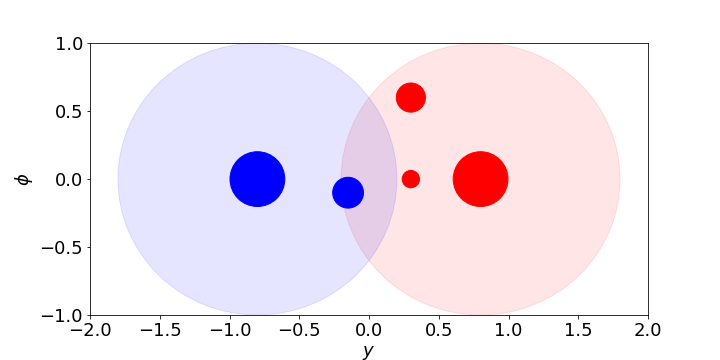
\includegraphics[width=0.8\textwidth]{antiktcls.png}
\end{center}
\end{frame}
%
%%%%%%%%%%%%%%%%%%%%%%%%%%%%%%%%%%%%%%%%%%%%%%%%%%%%%%%%%%
%
\begin{frame}\vspace{2mm}

{\color{darkred}\Large$\bullet$} {Simulations using a MC event generator (Herwig):}

\begin{center}
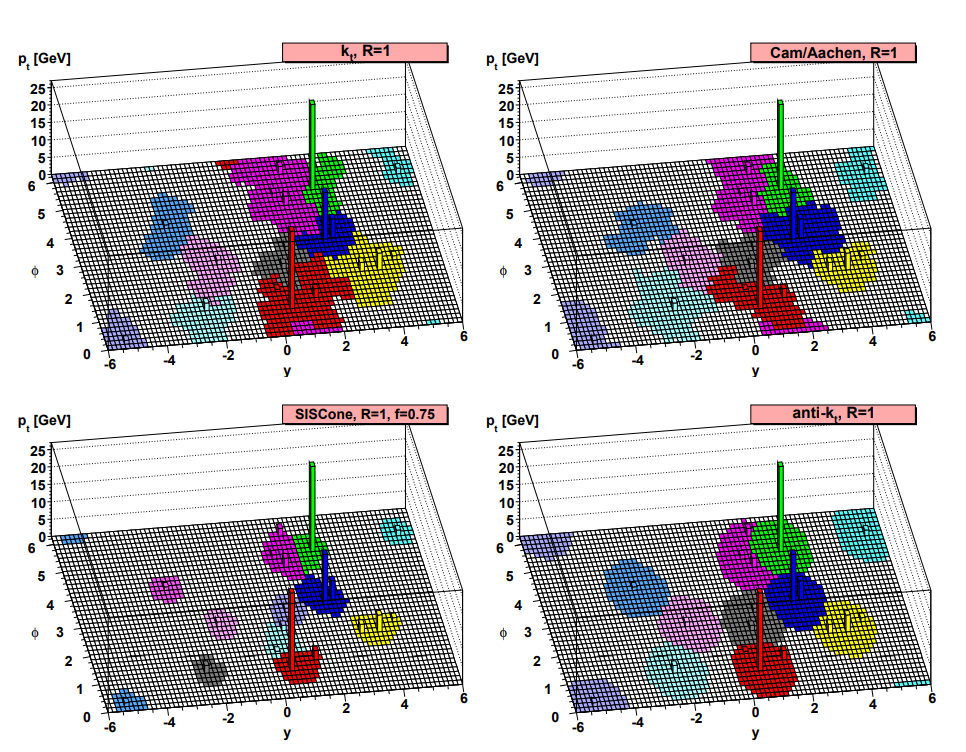
\includegraphics[width=0.8\textwidth]{03/algorithms.png}\\\vspace{2mm}

{\color{darkred}HW3: Cluster jets from $(p_T, y, \phi) = &(100, 0.8, 0), (100, -0.8, 0), (1, 0.2, -0.3), (1, 0.3, 0), (10, -0.15, -0.1), (8, 0.3, 0.6).$}
\end{center}
\end{frame}
%
%%%%%%%%%%%%%%%%%%%%%%%%%%%%%%%%%%%%%%%%%%%%%%%%%%%%%%%%%%
%
\begin{frame}{\bf\huge Infrared and collinear safety}

{\color{darkred}\Large$\bullet$} Infrared and collinear safety is required for sensible perturbative QCD calculations: \\
\vspace{2mm}
\vspace{2mm}
\begin{center}
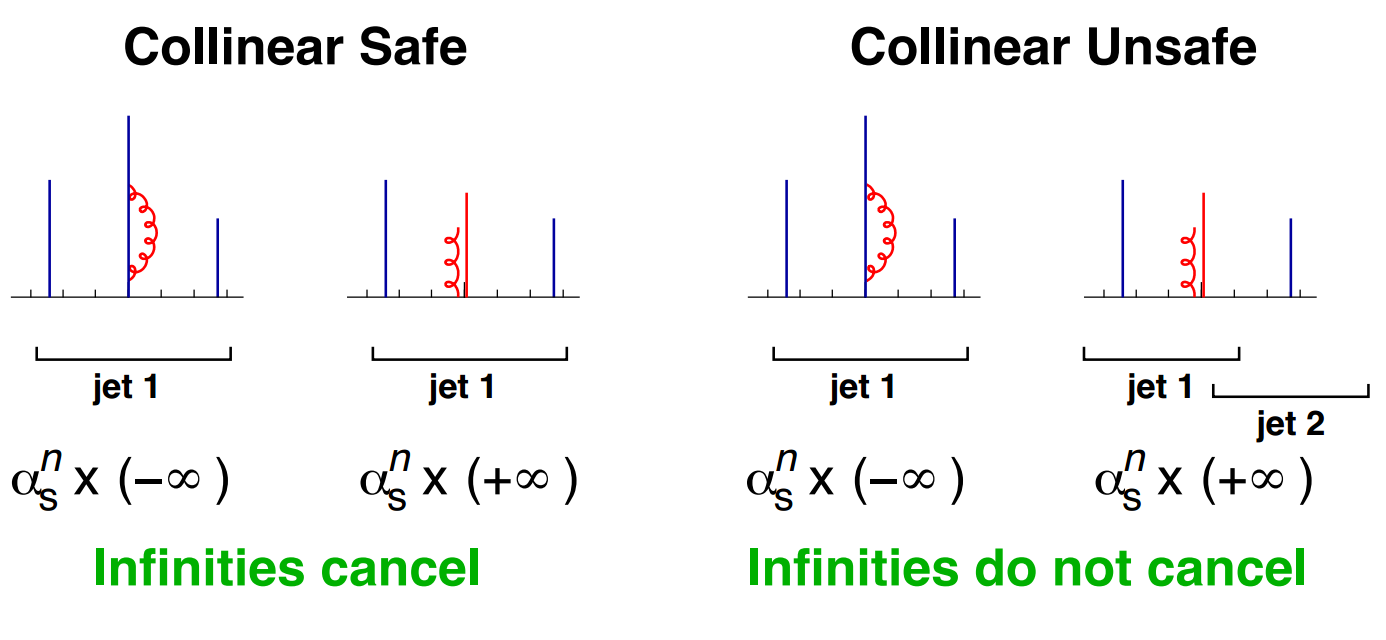
\includegraphics[width=\textwidth]{03/IRC.png}
\end{center}
\vspace{2mm}

{\color{darkred}\Large$\bullet$} Anti-$k_T$ is obviously collinear safe.
\end{frame}
%
%%%%%%%%%%%%%%%%%%%%%%%%%%%%%%%%%%%%%%%%%%%%%%%%%%%%%%%%%%
%
\begin{frame}

{\color{darkred}\Large$\bullet$} Is anti-$k_T$ infrared safe?\\
\vspace{2mm}
\begin{center}
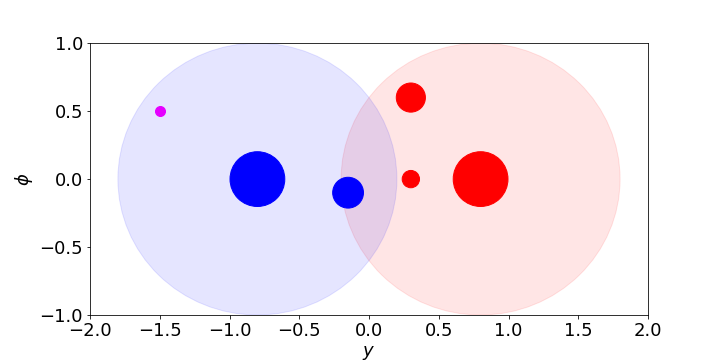
\includegraphics[width=\textwidth]{03/antiktSIn.png}
\end{center}
\end{frame}
%
%%%%%%%%%%%%%%%%%%%%%%%%%%%%%%%%%%%%%%%%%%%%%%%%%%%%%%%%%%
%
\begin{frame}

{\color{darkred}\Large$\bullet$} Is anti-$k_T$ infrared safe?\\
\vspace{2mm}
\begin{center}
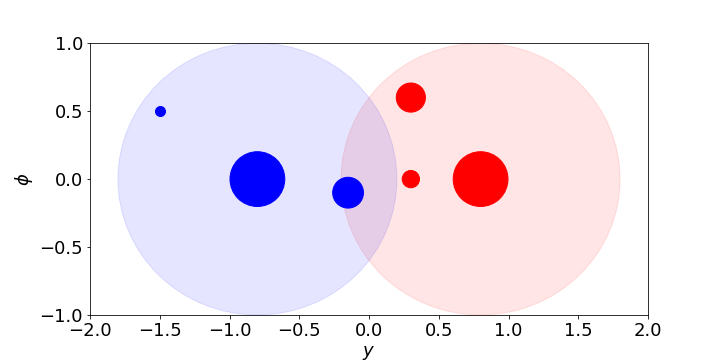
\includegraphics[width=\textwidth]{03/antiktS.png}
\end{center}
\end{frame}
%
%%%%%%%%%%%%%%%%%%%%%%%%%%%%%%%%%%%%%%%%%%%%%%%%%%%%%%%%%%
%
\begin{frame}

{\color{darkred}\Large$\bullet$} Is anti-$k_T$ infrared safe?\\
\vspace{2mm}
\begin{center}
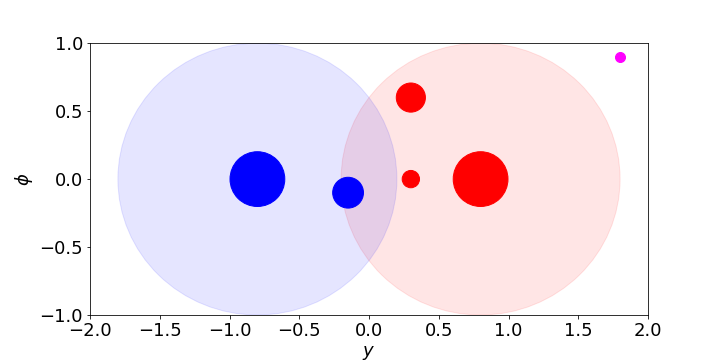
\includegraphics[width=\textwidth]{03/antiktSOut.png}
\end{center}
\end{frame}
%
%%%%%%%%%%%%%%%%%%%%%%%%%%%%%%%%%%%%%%%%%%%%%%%%%%%%%%%%%%
%
\begin{frame}

{\color{darkred}\Large$\bullet$} Is anti-$k_T$ infrared safe?\\
\vspace{2mm}
\begin{center}
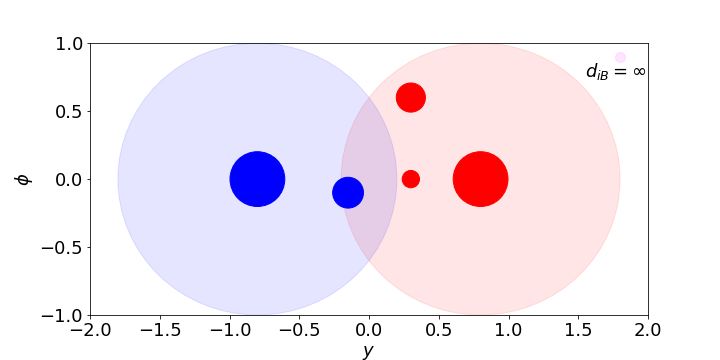
\includegraphics[width=\textwidth]{03/antiktSO.png}
\end{center}
\end{frame}
%
%%%%%%%%%%%%%%%%%%%%%%%%%%%%%%%%%%%%%%%%%%%%%%%%%%%%%%%%%%
%
\begin{frame}{\bf\huge Jet algorithms as optimization problem}\vspace{2mm}

{\color{darkred}\Large$\bullet$} {Several groups have considered jets as optimization problems.} \\
\vspace{2mm}

{\color{darkred}\Large$\bullet$} One approach: {\color{darkred} N-jettiness} \\
\vspace{2mm}
\begin{center}
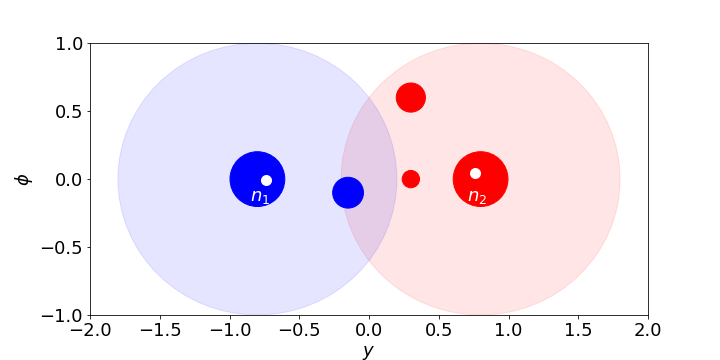
\includegraphics[width=0.7\textwidth]{03/njittiness.png}
\end{center}
Let us find exactly $N$ jets with axes $n_1, n_2, \cdots, n_N$. We want to find the optimal choice for $n_i$'s for the hardest $N$ jets. One way to do this (N-jettiness) is to minimize a penalty function:
\begin{align}
\tau_N =\sum\limits_{i\in\text{the list}}\text{min}\left\{p_{T,i }, p_{T,i } \left(\frac{\Delta R_{i n_1}}{R}\right)^2, \cdots, p_{T, i} \left(\frac{\Delta R_{i n_N}}{R}\right)^2 
\right\}.
\end{align}
\end{frame}
%
%%%%%%%%%%%%%%%%%%%%%%%%%%%%%%%%%%%%%%%%%%%%%%%%%%%%%%%%%%
%
\begin{frame}{\bf\huge Jet algorithms as optimization problem}\vspace{2mm}

{\color{darkred}\Large$\bullet$} {Example: 1-jettiness: assume all the particles are in the jet cone} \\
\vspace{2mm}
\begin{align}
    \tau_1 = \sum\limits_{i\in\text{the list}} p_{T, i} \left(\frac{\Delta R_{i1}}{R}\right)^2.
\end{align}
The local extremum is given by
\begin{align}
    \frac{\partial}{\partial \phi_{n_1}}\tau_1 = 0 = \frac{\partial}{\partial y_{n_1}}\tau_1,
\end{align}
that is,
\begin{align}
\phi_{n_1} = \frac{\sum\limits_i p_{T, i} \phi_i}{\sum\limits_i p_{T, i}}\qquad y_{n_1} = \frac{\sum\limits_i p_{T, i} y_i}{\sum\limits_i p_{T, i}}.
\end{align}

\end{frame}
\end{document}